\tikzstyle{kerros} = [rectangle, draw=black, rounded corners, minimum width=12cm, minimum height=1cm, text centered, font=\normalsize, line width=1]
\tikzstyle{palikka} = [rectangle, draw=black, minimum width=2.5cm, minimum height=1cm, text centered, font=\normalsize, line width=1, align=center]
\tikzstyle{nuoli} = [thick, draw=black, line width=1, ->, >=stealth]
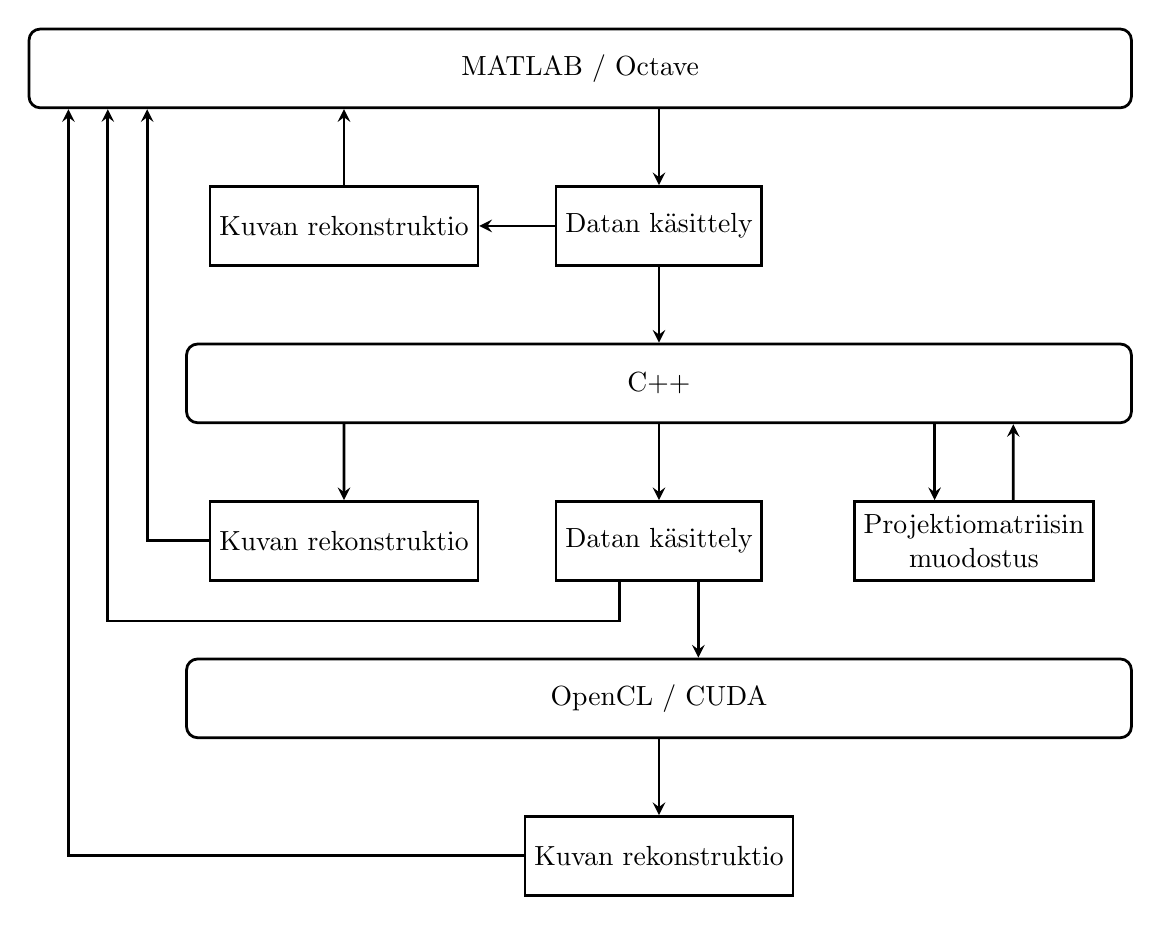
\begin{tikzpicture}[node distance=2cm]
    \node (kerros1) [kerros, minimum width=14cm] {MATLAB / Octave};
    \node (käsittely1) [below of=kerros1, xshift=1cm, palikka] {Datan käsittely};
    \node (rekonstruktio1) [left of=käsittely1, xshift=-2cm, palikka] {Kuvan rekonstruktio};
    
    \node (kerros2) [below of=käsittely1, kerros] {C++};
    \node (käsittely2) [below of=kerros2, palikka] {Datan käsittely};
    \node (projektiomatriisi) [right of=käsittely2, xshift=2cm, palikka] {Projektiomatriisin\\muodostus};
    \node (rekonstruktio2) [left of=käsittely2, xshift=-2cm, palikka] {Kuvan rekonstruktio};
    
    \node (kerros3) [below of=käsittely2, kerros] {OpenCL / CUDA};
    \node (rekonstruktio3) [below of=kerros3, palikka] {Kuvan rekonstruktio};
    
    \draw [nuoli] ([xshift=1cm]kerros1.south) -- (käsittely1);
    \draw [nuoli] (käsittely1) -- (kerros2);
    \draw [nuoli] (käsittely1) -- (rekonstruktio1);
    \draw [nuoli] (rekonstruktio1) -- ([xshift=-3cm]kerros1.south);

    \draw [nuoli] ([xshift=3.5cm]kerros2.south) -- ([xshift=-.5cm]projektiomatriisi.north);    
    \draw [nuoli] ([xshift=.5cm]projektiomatriisi.north) -- ([xshift=4.5cm]kerros2.south);
    \draw [nuoli] ([xshift=-4cm]kerros2.south) -- (rekonstruktio2);
    \draw [nuoli] (kerros2.south) -- (käsittely2);
    \draw [nuoli] ([xshift=.5cm]käsittely2.south) -- ([xshift=.5cm]kerros3.north);
    \draw [nuoli] (rekonstruktio2.west) -| ([xshift=-5.5cm]kerros1.south);
    \draw [nuoli] ([xshift=-.5cm]käsittely2.south) |- ([yshift=-.5cm]rekonstruktio2.south) -| ([xshift=-6cm]kerros1.south);

    \draw [nuoli] (kerros3) -- (rekonstruktio3);
    \draw [nuoli] (rekonstruktio3.west) -| ([xshift=-6.5cm]kerros1.south);
\end{tikzpicture}